\documentclass[8pt,a4paper]{article}
\usepackage[utf8]{inputenc}
\usepackage{lmodern,textcomp}
\usepackage[spanish]{babel}

\usepackage{amsmath}
\usepackage{amsfonts}
\usepackage{amssymb}

\usepackage{graphicx} %
\usepackage{multicol}
\usepackage[margin=1.4cm]{geometry}
\usepackage{url}
\usepackage{systeme} %Para alinear sistemas de ecuaciones

\usepackage{amsthm}
\pagenumbering{gobble}

\begin{document}

	\begin{center}
				\textbf{Matemáticas VI}\\
				Guía de la unidad 1: Matrices y determinantes \\
				Profesora Olivia Palma Avendaño
				\bigskip
	\end{center}
	
\paragraph*{Preámbulos} Esta guía servirá para definir la evaluación del último parcial y se entrega de manera remota en PDF; resuélvanla indicando sus procedimientos detalladamente. Apóyense de la lista de libros que les subí a Classroom; particularmente:

	\begin{enumerate}
		\item Edward T. Dowling - \textit{Schaum's Outline Theory and Problems of Introduction to Mathematical Economics}, capítulos 10 y 11.
		\item Robert Blitzer - \textit{College Algebra}, capítulos 5 y 6.
	\end{enumerate}

Pueden verificar las respuestas de los sistemas de ecuaciones utilizando el código del siguiente enlace:
	
	\begin{center}
		\url{https://repl.it/@mijamon/Sistemas-de-ecuaciones-lineales}
	\end{center}

También pueden escribirme si tienen dudas o necesitan ayuda.

	\begin{enumerate}

		\item Un hípermercado quiere ofertar tres clases de bandejas:  $A$, $B$ y $C$.  La bandeja $A$ contiene $40 g$ de queso manchego, $160 g$ de roquefort y $80 g$ de camembert; la bandeja $B$ contiene $120 g$ de cada uno de los tres tipos de queso anteriores; y la bandeja $C$, contiene $150 g$ de queso manchego, $80 g$ de roquefort y $80 g$ de camembert. Si se quiere sacar a la venta $50$ bandejas del tipo $A$, $80$ de $B$ y $100$ de $C$, obtén matricialmente la cantidad que necesitarán, en kilogramos, de cada una de las tres clases de quesos.

		\item Estudia para qué valores de $\lambda$ existe la inversa de la siguiente matriz:
%		
			\[A=\begin{pmatrix}
				1 & 1 & 1 \\
				\lambda & 0 & 2\\
				2 & -1 & 0
			\end{pmatrix}\]
%			
Calcula $A^{-1}$ para $\lambda=0$.

		\item Expresa y resuelve el siguiente sistema de forma matricial (OBR):

			\[ \systeme{x-2y+2z=0,-x+y-z=1, 2x+y=4}\]
			
		\item Tres personas $A$, $B$, $C$ quieren comprar las siguientes cantidades de fruta:
%
			\begin{itemize}
				\item[$A$:] 2 kg de peras, 1 kg de manzanas y 6 kg de naranjas.
				\item[$B$:] 2 kg de peras, 2 kg de manzanas y 4 kg de naranjas.
				\item[$C$:] 1 kg de peras, 2 kg de manzanas y 3 kg de naranjas.
			\end{itemize}
%			
En el pueblo en donde viven hay dos fruterías: $F_1$ y $F_2$. En $F_1$ las peras cuestan $1.5 €/kg$, las manzanas $1 €/kg$ y las naranjas $2 €/kg$. En $F_2$ las peras cuestan $1.8 €/kg$, las manzanas $0.8 €/kg$ y las naranjas $2.20 €/kg$.

			\begin{itemize}
				\item Expresa matricialmente la cantidad de fruta (peras, manzanas y naranjas) que quiere comprar cada persona $(A, B, C)$.
				\item Escribe una matriz con los precios de cada tipo de fruta en cada una de las dos fruterías.
				\item Obtén una matriz, a partir de las dos anteriores, en la que quede reflejado lo que se gastaría cada persona haciendo su compra en cada una de las dos fruterías.
			\end{itemize}
			
		\item Halla una matriz $B$, sabiendo que su primera fila es $(1, 0)$, y que verifica:
%
			\[A\cdot B=\begin{pmatrix}
						1 & 0 \\
						1 & 0
						\end{pmatrix}\]
siendo $\displaystyle A=\begin{pmatrix} -1 & 2 & 2 \\ 2 & 1 & 0 \end{pmatrix}$.

		\item Expresa en forma matricial y resuelve, utilizando la matriz inversa:
%
			\[ \systeme{3x+y-2z=1,x+2y+z=5,-2x+4y-2=3} \]
%
		\item Tres familias $A$, $B$, y $C$ van a ir de vacaciones a una ciudad en la que hay tres hoteles, $H_1$, $H_2$ y $H_3$. La familia $A$ necesita 2 habitaciones dobles y 1 sencilla; la familia $B$ necesita 3 habitaciones dobles y 1 sencilla; y la familia $C$ necesita 1 habitación doble y 2 sencillas. En el hotel $H_1$ el precio de la habitación doble es de $84 €/\text{día}$, y el de la habitación sencilla es de $45 €/\text{día}$. En $H_2$ la habitación doble cuesta $86 €/\text{día}$ y la sencilla cuesta $43 €/\text{día}$. En $H_3$ la doble cuesta $85 €/\text{día}$ y la sencilla cuesta $44 €/\text{día}$.
		
		\begin{itemize}
			\item Escribe en forma de matriz el número de habitaciones (dobles o sencillas) que necesita cada una de las tres familias.
			\item Expresa matricialmente el precio de cada tipo de habitación en cada uno de los tres hoteles.
			\item Obtén, a partir de las dos matrices anteriores, una matriz en la que se refleje el gasto diario que tendría cada una de las tres familias en cada uno de los tres hoteles.
		\end{itemize}

		\item Si $m,n\in\mathbb{N}$ son enteros no nulos, \textbf{una matriz $\mathbf{A}$ de $m\times n$} (o de $m$ renglones y $n$ columnas) es un arreglo rectangular de números reales $a_{ij}$ (llamados \textit{entradas de la matriz}) con la siguiente forma:
%		
			\[\mathbf{A}=\begin{pmatrix}
							a_{11} & a_{12} & \cdots & a_{1n} \\
							a_{21} & a_{22} & \cdots & a_{2n} \\
							\vdots & \vdots & \ddots & \vdots \\
							a_{m1} & a_{m2} & \cdots & a_{mn}
						\end{pmatrix}=\left(a_{ij}\right)\]
%
	Estos objetos se pueden operar de la siguiente manera:
	
		\begin{enumerate}
			\item \textbf{Multiplicación de matriz por escalar}:
				\[
				\lambda \mathbf{A}:=
					\begin{pmatrix}
							\lambda a_{11} & \lambda a_{12} & \cdots & \lambda a_{1n} \\
							\lambda a_{21} & \lambda a_{22} & \cdots & \lambda a_{2n} \\
							\vdots & \vdots & \ddots & \vdots \\
							\lambda a_{m1} & \lambda a_{m2} & \cdots & \lambda a_{mn}
					\end{pmatrix}=\left(\lambda a_{ij}\right)
				\]
			\item \textbf{Suma de matrices} (con el mismo número de renglones y columnas):
				\[
				\mathbf{A}+\mathbf{A}':=\begin{pmatrix}
							a_{11}+a_{11}' & a_{12}+a_{12}' & \cdots & a_{1n}+a_{1n}' \\
							a_{21}+a_{21}' & a_{22}+a_{22}' & \cdots & a_{2n}+a_{2n}' \\
							\vdots & \vdots & \ddots & \vdots \\
							a_{m1}+a_{m1}' & a_{m2}+a_{m2}' & \cdots & a_{mn}+a_{mn}'
						\end{pmatrix}=\left(a_{ij}+a_{ij}'\right)
				\]
			\item \textbf{Transposición de matrices}: \textit{convertir los renglones en columnas para obtener una matriz de $n\times m$}.
				\[
				\mathbf{A}^t:=
					\begin{pmatrix}
							a_{11} & a_{21} & \cdots & a_{m1} \\
							a_{12} & a_{22} & \cdots & a_{m2} \\
							\vdots & \vdots & \ddots & \vdots \\
							a_{1n} & a_{2n} & \cdots & a_{mn}
					\end{pmatrix}=\left(a_{ji}\right)
				\]
		\end{enumerate}
		
Por ejemplo: $\mathbf{A}=\begin{pmatrix} 1 & 5 & -3 \\ 0 & 3 & 2 \end{pmatrix}$, $\mathbf{A}'=\begin{pmatrix} 3 & 0 & -1 \\ 1 & -1 & 0 \end{pmatrix}$ son dos matrices de $2\times3$. Cada una de ellas tiene 6 elementos en total que se identifican con el renglón y columna donde se localizan, v.gr. el elemento del segundo renglón y tercera columna de $\mathbf{A}$ es $a_{23}=2$. Además:
%
	\begin{gather*}
		2\mathbf{A}'-\mathbf{A}=\begin{pmatrix} 2\cdot 3 & 2\cdot 0 & 2\cdot (-1) \\ 2\cdot 1 & 2\cdot (-1) & 2\cdot 0 \end{pmatrix}-\begin{pmatrix} 1 & 5 & -3 \\ 0 & 3 & 2 \end{pmatrix}=\begin{pmatrix} 6-1 & 0-5 & -2-(-3) \\ 2-0 & -2-3 & 0-2 \end{pmatrix}=\begin{pmatrix} 5 & -5 & 1 \\ 2 & -5 & -2	\end{pmatrix}, \\
		\mathbf{A}^t=\begin{pmatrix} 1 & 0 \\ 5 & 3 \\ -3 & 2 \end{pmatrix}.
	\end{gather*}
%
Dadas $\displaystyle \mathbf{A}:=\begin{pmatrix} 2 & 1 \\ 3 & -3 \\ -1 & 3 \end{pmatrix}$, $\displaystyle \mathbf{B}:=\begin{pmatrix} 2 & 1 & 3 \\ -3 & -1 & 3 \end{pmatrix}$, $\displaystyle \mathbf{C}:=\begin{pmatrix} 0 & 5 \\ 1 & 0 \\ -3 & 2 \end{pmatrix}$, calcula:

	\begin{multicols}{2}
		\begin{itemize}
			\item $\displaystyle 3\mathbf{A}+2\mathbf{B}^t$
			\item $\displaystyle \mathbf{B}-\mathbf{C}^t$
			\item $\displaystyle \left(-\mathbf{A}^t+3\mathbf{B}\right)^t$
			\item $\displaystyle \left(\mathbf{A}+\mathbf{B}^t+\mathbf{C}\right)^t$
			\item $\displaystyle \left(\mathbf{A}^t\right)^t$
			\item $\displaystyle \mathbf{A}^t+\mathbf{B}+\mathbf{C}^t$
		\end{itemize}
	\end{multicols}
	
		\item ¿Por qué es cierto que $\left(\mathbf{A}^t\right)^t=\mathbf{A}$? Explica con detalle.
	
		\item A las matrices de $n$ renglones y $1$ columna se les llama \textit{vectores columna}, y se les suele representar con letras minúsculas:
%		
		\[\mathbf{a}=\begin{pmatrix} a_1 \\ \vdots \\ a_n \end{pmatrix}.\]
%
(Dado que sólo tienen una columna, no hace falta representar sus entradas con dos subíndices). Un \textit{vector renglón} es la transposición de un vector columna $\mathbf{a}$: $\mathbf{a}^t$. \textbf{El producto interior de un vector renglón por un vector columna} es:
%
		\[\mathbf{a}^t\mathbf{b}=\begin{pmatrix} a_1 & a_2 & \cdots & a_n \end{pmatrix} \begin{pmatrix} b_1 \\ b_2 \\ \vdots \\ b_n \end{pmatrix}:=a_1\cdot b_1+a_2\cdot b_2+\cdots+a_n\cdot b_n.\]
%
(Hay que resaltar que el número de columnas del vector renglón debe coincidir con el número de renglones del vector columna).

Por ejemplo:
%
		\[\begin{pmatrix} 1 & -3 & 2 \end{pmatrix}\begin{pmatrix} -1 \\ 1 \\ 2 \end{pmatrix}=1\cdot(-1)+(-3)\cdot 1+2\cdot 2=-1-3+4=0.\]
%
Dados $\displaystyle \mathbf{x}^t=\begin{pmatrix}1 & -1 & 0\end{pmatrix}, \mathbf{y}^t=\begin{pmatrix}2 & 1 & 3\end{pmatrix}, \mathbf{z}^t=\begin{pmatrix}2&4&-2\end{pmatrix}$, calcula:

	\begin{multicols}{2}
		\begin{itemize}
			\item $\displaystyle 3\mathbf{x}^t\left(2\mathbf{y}\right)$
			\item $\displaystyle \mathbf{y}^t\mathbf{y}$
			\item $\displaystyle \mathbf{z}^t\left(-\mathbf{x}\right)$
			\item $\displaystyle \mathbf{x}^t\mathbf{x}+\mathbf{y}^t\mathbf{y}+\mathbf{z}^t\mathbf{z}$
			\item $\displaystyle \mathbf{y}^t\left(\mathbf{x}-\mathbf{z}\right)$
			\item $\displaystyle \left(\mathbf{x}^t-\mathbf{z}^t\right)\mathbf{y}$
		\end{itemize}
	\end{multicols}
	
		\item Dos matrices de dimensiones $r_1\times c_1$ y $r_2\times c_2$ son \textit{conformes} si $c_1=r_2$, es decir, si el número de columnas de la primera es igual al número de renglones de la segunda. Por ejemplo, si:
%
		\[	\mathbf{A}:=
			\begin{pmatrix}
				3 & 6 & 7 \\
				12 & 9 & 11
			\end{pmatrix}_{2\times 3},\;
			\mathbf{B}:=
			\begin{pmatrix}
				6 & 12 \\
				5 & 10 \\
				13 & 2
			\end{pmatrix}_{3\times 2},\;
			\mathbf{C}:=
			\begin{pmatrix}
				1 & 7 & 8 \\
				2 & 4 & 3
			\end{pmatrix}_{2\times 3}
		\]
%
entonces $\mathbf{A}$ es conforme con $\mathbf{B}$, $\mathbf{B}$ es conforme con $\mathbf{C}$ y $\mathbf{C}$ es conforme con $\mathbf{B}$; hay que notar también que $\mathbf{A}$ no es conforme con $\mathbf{C}$ ni $\mathbf{C}$ es conforme con $\mathbf{A}$.

	En las matrices anteriores se colocaron subíndices para indicar sus dimensiones, con la finalidad de analizar la conformidad entre ellas. \textbf{El producto de matrices conformes} se define con la ayuda del producto interior de vectores renglón y columna. Por ejemplo, podemos reescribir las matrices $\mathbf{A}$ y $\mathbf{B}$ de antes en términos de renglones y columnas:
%
		\[ \mathbf{A}=\begin{pmatrix} R_1 \\ R_2 \end{pmatrix}, \;
		\mathbf{B}=\begin{pmatrix} C_1 & C_2 \end{pmatrix}\]
%
donde $R_1=\begin{pmatrix}3 & 6 & 7\end{pmatrix}$, $R_2=\begin{pmatrix}12 & 9 & 11\end{pmatrix}$, $C_1=\begin{pmatrix}6 \\ 5 \\ 13 \end{pmatrix}$, $C_2=\begin{pmatrix} 12 \\ 10 \\ 2 \end{pmatrix}$. Su producto o multiplicación matricial es:
%
	\[\mathbf{A}\mathbf{B}=\begin{pmatrix}
							R_1C_1 & R_1C_2  \\
							R_2C_1 & R_2C_2 \\
							\end{pmatrix}
						=\begin{pmatrix}
							3(6)+6(5)+7(13) & 3(12)+6(10)+7(2) \\
							12(6)+9(5)+11(13) & 12(12)+9(10)+11(2)
						\end{pmatrix}
						=\begin{pmatrix}
							139 & 110 \\
							260 & 256
						\end{pmatrix}_{2\times 2}
	\]
%
	En general, si $\mathbf{A}=\left(a_{ij}\right), \mathbf{B}=\left(b_{ij}\right)$ son matrices conformes de dimensión $r_1\times n$, $n \times c_2$, respectivamente, su producto $\mathbf{AB}$ será una matriz de dimensión $r_1\times c_2$ con entradas:
%
	\[\mathbf{AB}=\left(\sum_{k=1}^n a_{ik}b_{kj}\right)\]
%
		\begin{enumerate}
			\item Calcula $\mathbf{AB}$ y $\mathbf{BA}$ para los siguientes pares de matrices:
%
			\begin{multicols}{2}
				\begin{itemize}
					\item $\displaystyle \mathbf{A}=\begin{pmatrix} 1 & 1 & 1 & 1 \end{pmatrix},\;
										\mathbf{B}=\begin{pmatrix} 1 \\ 1 \\ 1 \\ 1 \end{pmatrix}$;
					\item $\displaystyle \mathbf{A}=\begin{pmatrix} 4 & 7 \\ 2 & 6 \\ 8 & 1 \end{pmatrix},\;
										\mathbf{B}=\begin{pmatrix} 2 & 12 & 7 \\ -1 & 3 & 1 \end{pmatrix}$;
					\item $\displaystyle \mathbf{A}=\begin{pmatrix} 1 & 12 & 13 \\ 1 & 3 & 6 \end{pmatrix},\;
										\mathbf{B}=\begin{pmatrix} 7 & 5 \\ 4 & 7 \\ 1 & 3 \end{pmatrix}$;
					\item $\displaystyle \mathbf{A}=\begin{pmatrix} 1 & 0 & 0 \\ 0 & 1 & 0 \\ 0 & 0 & 1 \end{pmatrix},\;
										\mathbf{B}=\begin{pmatrix} 1 & 2 & 8 \\ 7 & 6 & 2 \\ 0 & 2 & 4 \end{pmatrix}$.
				\end{itemize}
			\end{multicols}
%
¿Es cierto que el producto de matrices es conmutativo? Explica.
			\item Calcula el producto $\mathbf{Ax}$ para las siguientes matrices:
				\begin{multicols}{2}
				\begin{itemize}
					\item $\displaystyle \mathbf{A}=\begin{pmatrix} 1 & 0 & 0 \\ 0 & 1 & 0 \\ 0 & 0 & 1 \end{pmatrix},
											\mathbf{x}=\begin{pmatrix} 1 \\ -1 \\ 1 \end{pmatrix}$;
					\item $\displaystyle \mathbf{A}=\begin{pmatrix} 2 & 0 & 5 \\ 3 & 4 & 1 \\ 7 & 9 & 6 \end{pmatrix},
											\mathbf{x}=\begin{pmatrix} 5 \\ 4 \\ 6 \end{pmatrix}$;
					\item $\displaystyle \mathbf{A}=\begin{pmatrix} 3 & 13 \\ 7 & 9 \\ 2 & 1 \\ 8 & 6 \end{pmatrix},
											\mathbf{x}=\begin{pmatrix} 1 \\ -1 \end{pmatrix}$;
					\item $\displaystyle \mathbf{A}=\begin{pmatrix} 0 & 0 & 0 & 1 \\ 0 & 0 & 1 & 0 \\
																	0 & 1 & 0 & 0 \\1 & 0 & 0 & 0 \end{pmatrix},
											\mathbf{x}=\begin{pmatrix} 1 \\ -1 \\ 0 \\ 1 \end{pmatrix}$.
				\end{itemize}
				\end{multicols}
		\end{enumerate}
		
		\item Resuelve los siguientes sistemas de ecuaciones para las incógnitas $x,y$ mediante el método de suma y resta.
		
			\begin{multicols}{2}
				\begin{enumerate}
					\item $\displaystyle \systeme{7x-3y=8, 4x+9y=-24}$
					\item $\displaystyle \systeme{4x+\frac{9}{y}=21,\frac{18}{y}=17-3x}$
					\item $\displaystyle \systeme{\frac{x}{a}+\frac{y}{b}=1,\frac{x}{b}-\frac{y}{a}=1}$
					\item $\displaystyle \systeme{\frac{x}{a+b}+\frac{y}{a-b}=2a, x-y=4ab}$
				\end{enumerate}
			\end{multicols}	

		\item Resuelve los siguientes sistemas de ecuaciones utilizando matrices aumentadas y el método de reducción de Gauss-Jordan.
		
			\begin{multicols}{2}
				\begin{enumerate}
					\item $\displaystyle \systeme*{2x-y+z=3, x+3y-2z=11, 3x-2y+4z=1}$
					\item $\displaystyle \systeme*{\frac{x}{3}+\frac{y}{2}-\frac{z}{4}=2,
							\frac{x}{4}+\frac{y}{3}-\frac{z}{2}=\frac{1}{5},
							\frac{x}{2}-\frac{y}{4}+\frac{z}{3}=\frac{23}{6}}$
					\item $\displaystyle \systeme*{\frac{1}{x}-\frac{2}{y}-\frac{2}{z}=0,
							\frac{2}{x}+\frac{3}{y}+\frac{1}{z}=1,
							\frac{3}{x}-\frac{1}{y}-\frac{3}{z}=3}$
					\item $\displaystyle \systeme*{3x+y-z=4,x+y+4z=3,9x+5y+10z=8}$
				\end{enumerate}
			\end{multicols}
			
		\item Además de la representación de un sistema de ecuaciones lineales mediante la matriz aumentada, podemos usar el producto de matrices rectangulares por vectores columna. Por ejemplo, el sistema:
%		
			\[\systeme*{4x_1+x_2-5x_3=8,-2x_1+3x_2+x_3=12,3x_1-x_2+4x_3=5}\]
%
puede reescribirse como:
%
			\[\begin{pmatrix}
				4 & 1 & -5 \\
				-2 & 3 & 1 \\
				3 & -1 & 4
				\end{pmatrix}\begin{pmatrix}x_1\\x_2\\x_3\end{pmatrix}=\begin{pmatrix}8\\12\\5\end{pmatrix}\]
%
Representa de esta manera los sistemas de ecuaciones del problema anterior.

		\item Supón que las funciones de oferta y demanda de un bien están dadas, respectivamente, por:
%
			\[\systeme*{x_1=2+2x_2,x_1=4-4x_2}\]
%
donde $x_1$ representa la cantidad y $x_2$ el precio. ¿Cuáles son la cantidad y el precio que resuelven el sistema?

		\item De manera muy parecida al conjunto de números reales $\mathbb{R}$, sus operaciones $+,\cdot$ y sus neutros $0,1$, las matrices también cumplen propiedades de asociatividad, conmutatividad y existencia de un elementro para la operación de suma; de asociatividad para el producto de matrices conformes; y de distributividad del producto respecto a la suma. Lista todas estas propiedades y discute \textbf{detalladamente} sus parecidos y diferencias con $\left(\mathbb{R},+,0,\cdot,1\right)$. ¿Cuál es el elemento neutro de la multiplicación de matrices cuadradas?

		\item Si $\mathbf{A}$ es una matriz de $2\times 2$, su \textbf{determinante} es el siguiente número:
%
	\[\mathrm{det}\left(\mathbf{A}\right)=\left|\mathbf{A}\right|=
		\begin{vmatrix} a_{11} & a_{12} \\ a_{21} & a_{22} \end{vmatrix}
		:=a_{11}a_{22}-a_{12}a_{21}
	\]
%
Por ejemplo:
%
	\[\mathrm{det}\begin{pmatrix} 1 & 2 \\ -5 & 3 \end{pmatrix}=
	\begin{vmatrix} 1 & 2 \\ -5 & 3 \end{vmatrix}=1\cdot 3 - 2(-5)=3+10=13
	\]
%
Calcula el determinante de las siguientes matrices:
	\begin{multicols}{3}
		\begin{itemize}
			\item $\displaystyle \begin{pmatrix} -2 & 3 \\ 5 & -1 \end{pmatrix}$;
			\item $\displaystyle \begin{pmatrix} 1 & 1 \\ 2 & 2 \end{pmatrix}$;
			\item $\displaystyle \begin{pmatrix} 3 & -7 \\ 4 & 1 \end{pmatrix}$;
			\item $\displaystyle \begin{pmatrix} -2 & 3 \\ 5 & -1 \end{pmatrix}$;
			\item $\displaystyle \begin{pmatrix} 0 & 1 \\ 1 & 0 \end{pmatrix}$;
			\item $\displaystyle \begin{pmatrix} \cos \alpha & -\sin \alpha \\ \sin \alpha & \cos \alpha \end{pmatrix}$ (con $\alpha\in\mathbb{R}$ fijo pero arbitrario).
		\end{itemize}
	\end{multicols}
		\item Considera el conjunto de matrices (cuadradas) de dimensión $n$:
%
			\[ \mathcal{M}_n(\mathbb{R}):=\{\mathbf{A}=(a_{ij}):a_{ij}\in\mathbb{R}; i,j=1,\dots,n\} \]
%
donde $n$ es un número fijo. En general, \textbf{el determinante} es la función $\mathrm{det}:\mathcal{M}_n(\mathbb{R})\longrightarrow\mathbb{R}$ que a cada matriz cuadrada $\mathbf{A}=(a_{ij})$ le asocia un número real $\mathrm{det}\left(\mathbf{A}\right)=\left|\mathbf{A}\right|$:
%
	\[
	\mathrm{det}\left(\mathbf{A}\right)=\left|\mathbf{A}\right|:=\sum_{\sigma\in S_n} 
		\left(\mathrm{sgn}(\sigma)\prod_{i=1}^n a_{i\sigma(i)}\right)
	\]
%
donde $S_n$ es el conjunto de todas las funciones biyectivas (o permutaciones) $\sigma$ de $\{1,2,\dots,n\}$, y $\mathrm{sgn}(\sigma)$ es $\pm 1$ dependiendo de si la permutación $\sigma$ tiene un número par o impar de trasposiciones, respectivamente. La \textbf{fórmula de Laplace} es una manera alternativa de calcular el determinante de una matriz cuadrada de manera recursiva:
%
\begin{align*}
(n=1) \hspace{6mm} \mathrm{det}\left(\mathbf{A}\right)&=a_{11}; \\
(n>1) \hspace{6mm} \mathrm{det}\left(\mathbf{A}\right)&=
		\sum_{j=1}^n (-1)^{i+j}a_{ij}\left|M_{ij}\right| \;(\text{desarrollo en renglón i})\\
		&=\sum_{i=1}^n (-1)^{i+j}a_{ij}\left|M_{ij}\right| \;\text{(desarrollo en columna j)},
\end{align*}
%
donde $M_{ij}$ es la matriz de dimensión $n-1$ que resulta al eliminar el renglón $i$ y la columna $j$\footnote{El número $(-1)^{i+j}\left|M_{ij}\right|$ es llamado \textit{cofactor} del elemento $a_{ij}$; en cambio, $\left|M_{ij}\right|$ se llama \textit{menor} del elemento $a_{ij}$}. Por ejemplo, desarrollando respecto a la segunda columna ($j=2$):
%
\begin{align*}
\mathrm{det}\begin{pmatrix}
				-2 & 2 & -3 \\
				-1 & 1 & 3 \\
				2 & 0 & -1
			\end{pmatrix} &= (-1)^{1+2}\cdot 2 \cdot \begin{vmatrix} -1 & 3 \\ 2 & -1 \end{vmatrix}
			+(-1)^{2+2}\cdot 1 \cdot \begin{vmatrix} -2 & -3 \\ 2 & -1 \end{vmatrix}
			+(-1)^{3+2}\cdot 0 \cdot \begin{vmatrix} -2 & -3 \\ -1 & 3 \end{vmatrix}\\
			&= (-2)\cdot\left((-1)\cdot(-1)-2\cdot 3\right)+1\cdot\left((-2)\cdot(-1)-2\cdot(-3)\right)\\
			&= (-2)(-5)+8=18.
\end{align*}
%
Y desarrollando respecto al primer renglón:
%
\begin{align*}
\mathrm{det}\begin{pmatrix}
				-2 & 2 & -3 \\
				-1 & 1 & 3 \\
				2 & 0 & -1
			\end{pmatrix} &= (-1)^{1+1}\cdot (-2) \cdot \begin{vmatrix} 1 & 3 \\ 0 & -1 \end{vmatrix}
			+(-1)^{1+2}\cdot 2 \cdot \begin{vmatrix} -1 & 3 \\ 2 & -1 \end{vmatrix}
			+(-1)^{1+3}\cdot (-3) \cdot \begin{vmatrix} -1 & 1 \\ 2 & 0 \end{vmatrix} \\
			&= (-2)\cdot \left( 1\cdot(-1)-3 \cdot 0 \right)-2 \left( (-1)\cdot(-1)-3\cdot 2\right)
				-3\left( (-1)\cdot 0 - 1\cdot 2 \right) \\
			&= (-2)(-1)-2(-5)-3(-2)=2+10+6=18
\end{align*}
\textit{Cualquier manera de desarrollar da el mismo resultado.}
	
	Calcula el determinante de las siguientes matrices mediante la fórmula de Laplace y respecto al renglón o columna indicado:
	\begin{multicols}{2}
		\begin{itemize}
			\item $\displaystyle \begin{pmatrix} -2 & 3 & 1 \\ 0 & 5 & -1 \\ 1 & 1 & 0 \end{pmatrix}$, columna 3;
			\item $\displaystyle \begin{pmatrix} 4 & 1 & -5 \\ -2 & 3 & 1 \\ 3 & -1 & 4 \end{pmatrix}$, renglón 3;
			\item $\displaystyle \begin{pmatrix} 12 & 7 & 0 \\ 6 & 7 & 0 \\ 5 & 8 & 3 \end{pmatrix}$, columna 1;
			\item $\displaystyle \begin{pmatrix} 8 & 3 & 2 \\ 5 & 1 & 3 \\ 6 & 4 & 7 \end{pmatrix}$, renglón 2;
			\item $\displaystyle \begin{pmatrix} 7 & 9 & 1 \\ 2 & 1 & 8 \\ 3 & 6 & 5 \end{pmatrix}$, renglón 1;
			\item $\displaystyle \begin{pmatrix} 0 & 6 & 0 \\ 3 & 5 & 2 \\ 7 & 6 & 9 \end{pmatrix}$, columna 2;
			\item $\displaystyle \begin{pmatrix} 2 & 5 & 8 & 3 \\ 3 & 10 & 2 & 1 
					\\ 2 & 4 & 7 & 1 \\ 1 & 15 & 0 & 4 \end{pmatrix}$, renglón 1.
		\end{itemize}
	\end{multicols}

		\item Investiga qué es la regla de Sarrus y aplícala para calcular el determinante de las matrices del problema anterior. ¿Puede usarse para matrices cuadradas de orden $n\geq 4$?

		\item Dada $\mathbf{A}\in\mathcal{M}_n(\mathbb{R})$, \textbf{su adjunta} es la transpuesta de la matriz formada por los cofactores:
%
			\[\textrm{Adj}(\mathbf{A}):=\left((-1)^{i+j}\det(M_{ij})\right)^t\]
%
(ver nota al pie del problema 11). Por ejemplo:
%
		\begin{align*}
		\mathrm{Adj}\begin{pmatrix} 2 & 3 & 1 \\ 4 & 1 & 2 \\ 5 & 3 & 4 \end{pmatrix}
		&=
		\begin{pmatrix}
			(-1)^{1+1}\begin{vmatrix}1&2\\3&4\end{vmatrix} & 
			(-1)^{1+2}\begin{vmatrix}4&2\\5&4\end{vmatrix} &
			(-1)^{1+3}\begin{vmatrix}4&1\\5&3\end{vmatrix} \\			
			(-1)^{2+1}\begin{vmatrix}3&1\\3&4\end{vmatrix} & 
			(-1)^{2+2}\begin{vmatrix}2&1\\5&4\end{vmatrix} &
			(-1)^{2+3}\begin{vmatrix}2&3\\5&3\end{vmatrix} \\
			(-1)^{3+1}\begin{vmatrix}3&1\\1&2\end{vmatrix} & 
			(-1)^{3+2}\begin{vmatrix}2&1\\4&2\end{vmatrix} &
			(-1)^{3+3}\begin{vmatrix}2&3\\4&1\end{vmatrix} 
		\end{pmatrix}^t
		=\begin{pmatrix}
		
		\end{pmatrix}
			-2 & -6 & 7 \\ -9 & 3 & 9 \\ 5 & 0 & -10
		\end{pmatrix}^t \\
		&=\begin{pmatrix}
			-2 & -9 & 5 \\- 6 & 3 & 0 \\ 7 & 9 & -10
		\end{pmatrix}
		\end{align*}
%
	Calcula la adjunta de cada una de las matrices del problema 11.

		\item Dado un sistema de $n$ ecuaciones lineales con $n$ incógnitas en forma matricial $\mathbf{Ax}=\mathbf{b}$, si $\det(\mathbf{A})\neq 0$ \textit{el sistema tiene solución}. Una manera de encontrarla explícitamente es mediante la matriz adjunta:
%
\[\mathbf{x}=\frac{1}{\det\mathbf{A}}\mathrm{Adj}\left(\mathbf{A}\right)\mathbf{b}\]
%
Por ejemplo, el sistema:
%
\[\systeme{4x_1+3x_2=28,2x_1+5x_2=42}\]
%
se puede representar como $\mathbf{Ax}=\mathbf{b}$, donde:
%
\[\mathbf{A}=\begin{pmatrix} 4 & 3 \\ 2 & 5 \end{pmatrix},\;\mathbf{b}=\begin{pmatrix} 28 \\ 42 \end{pmatrix}\]
%
Calculando la adjunta y el determinante de $\mathbf{A}$, tenemos:
%
\[\mathrm{Adj}(\mathbf{A})=\begin{pmatrix} 5 & -3 \\ -2 & 4 \end{pmatrix},\;\det\mathbf{A}=14.\]
%
Por lo tanto, la solución del sistema es:
%
\[\mathbf{x}=\frac{1}{14}\begin{pmatrix} 5 & -3 \\ -2 & 4 \end{pmatrix}\begin{pmatrix}28\\42\end{pmatrix}=
	\begin{pmatrix} 5 & -3 \\ -2 & 4 \end{pmatrix}\begin{pmatrix}2\\3\end{pmatrix}=\begin{pmatrix}10-9\\-4+12\end{pmatrix}
	=\begin{pmatrix}1\\8\end{pmatrix}\]
%
(es decir, $x_1=1,\,x_2=8$).
	Utilizando este método, encuentra la solución de los siguientes problemas:
		\begin{itemize}
			\item Precios de equilibrio de los mercados de carne de cerdo y res, con condiciones de equilibrio: 
			
			\[ \systeme{18P_r-P_c=87,-2P_r+36P_c=98};\]
			
			\item Nivel de ingresos $Y$ en equilibrio y tasa de de interés $i$, con condiciones de equilibrio: 
			
			\[ \systeme{0.35Y+95i-48=0,0.32Y-210i-183=0}; \]
			\item $\displaystyle \systeme{2x_1+4x_2-3x_3=12,3x_1-5x_2+2x_3=13,-x_1+3x_2+2x_3=17}$;
			\item Precio de equilibrio para tres mercados: $\displaystyle \systeme{11P_1-P_2-P_3=31,-P_1+6P_2-2P_3=26,-P_1-2P_2+7P_3=24}$.
		\end{itemize}
		
		\item La siguiente tabla muestra los resultados de un estudio que trata de relacionar tasa de mortalidad con tiempo de sueño:
		
		\begin{center}
			\begin{tabular}{c|c}
			$x$ & $y$ \\
			\hline
			4 & 1682 \\
			7 & 626 \\
			9 & 967
			\end{tabular}
		\end{center}
donde $x$ representa el número promedio de horas diarias de sueño y $y$ la tasa de mortalidad por cada $10,000$ hombres. Utiliza la función cuadrática $y=ax^2+bx+c$ para modelar estos datos. ¿Cuál es la tasa de mortalidad para hombres que duermen un promedio de 6 horas diarias? ¿Y para aquellos que duermen 8? (Recuerda que la interpolación de datos no siempre es lineal, así que \textit{usar regla de 3} es incorrecto.)

	\item Una compañía planea manufacturar lectores digitales de libros \textit{kobo}. El costo fijado es de $\textrm{USD}\$400,00$ y costará $\textrm{USD}\$20$ producir cada kobo. Se piensa vender cada uno en $\textrm{USD}\$100$.

		\begin{enumerate}
			\item ¿Cuál es la función $C=C(x)$ del costo de producción de $x$ kobos?
			\item ¿Cuál es la correspondiente función de ingresos $R=R(x)$?
			\item Escribe la función de las utilidades $P=P(x)$ de producir y vender $x$ kobos.
			\item ¿Cuál es el precio de equilibrio? ¿Qué significa este resultado?
		\end{enumerate}
	
	\item El administrador de un centro de jardinería necesita mezclar dos tipos de nutrientes para plantas con $13\%$ y $18\%$ de contenido de nitrógeno. ¿Cuántos galones de cada nutriente debe mezclar para obtener 50 galones al $15\%$ de nitrógeno?

	\item La siguiente tabla da una estimación de los requerimientos calóricos para distintos grupos etarios de acuerdo a su nivel de actividad física:
	
	\begin{center}
		\begin{tabular}{c|c|c|c}
			Rango de edad & Sedentario & Medio activo & Activo \\
			\hline
			19-30 & (H:2400, M:2000) & (H:2700, M:2100) & (H:3000, M:2400) \\
			31-50 & (H:2200, M:1800) & (H:2500, M:2000) & (H:2900, M:2200) \\
			51+	 & (H:2000, M:1600) & (H:2300, M:1800) & (H:2600, M:2100)
		\end{tabular}
	\end{center}
(en cada caso: H = hombre, M = mujer). Si $\mathbf{H}, \mathbf{M}$ son las matrices con los datos únicamente de hombre o mujer, ¿qué representa la matriz $\mathbf{H}-\mathbf{M}$?
	
	\item La siguiente figura muestra la intersección de tres vías de un solo sentido. Los números $x,y,z$ representan el flujo vial (medido en número de carros por hora) en hora pico.
	
		\begin{figure}[!h]
		\centering
		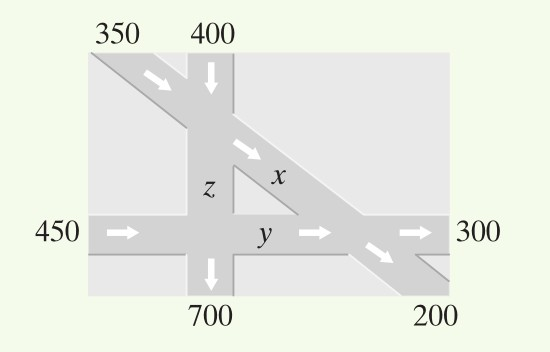
\includegraphics[scale=0.4]{trafico.jpg}
		\end{figure}

	\begin{enumerate}
		\item Si el número de carros que entran en cada intersección por cada hora debe ser igual al número de los que salen, ¿qué sistema de ecuaciones resulta?
		\item Utiliza el método de eliminación gaussiana para resolver el sistema.
		\item Si la construcción limita $z$ a 400, ¿cuántos carros por hora deben pasa entre las demás intersecciones para mantener el tránsito fluyendo?
	\end{enumerate}
	
	\end{enumerate}

\end{document}